

\documentclass{beamer}
\usepackage[utf8]{inputenc}
\usepackage[frenchb]{babel}
\usepackage[T1]{fontenc}
\usetheme{Darmstadt}
\usecolortheme{beaver}


\usepackage{pgfplots}

\usepackage{graphicx}


\title{Sparse Representation}
\author{Nicolas Lupinski \& Gregory Potdevin \& Rémy El Sibaïe Besognet}

\definecolor{light-gray}{gray}{0.80}

\begin{document}

\begin{frame}
  \titlepage  
\end{frame}


\begin{frame}{Introduction}

\begin{block}{Previous optimizations}
\begin{itemize}
\item 64 bits hash
\item small cardinalities : linear counting
\item no bias ($n < 65000$)
\end{itemize}
\end{block}


\begin{block}{Goals}
\begin{itemize}
\item Accuracy
\item Memory efficiency
\item \only<1>{Estimate large cardinalities} \only<2->{\textcolor{light-gray}{Estimate large cardinalities}}
\item \only<1>{Practicality} \only<2->{\textcolor{light-gray}{Practicality}}
\end{itemize}
\end{block}


\end{frame}

\begin{frame}{Why a sparse representation}

HyperLogLog uses a fixed amount of memory depending on the precision ($6\times m$ bits)

(idx : $log_2(m)$ bits, $\varrho(w)$ : 6 bits)

\begin{figure}[c]
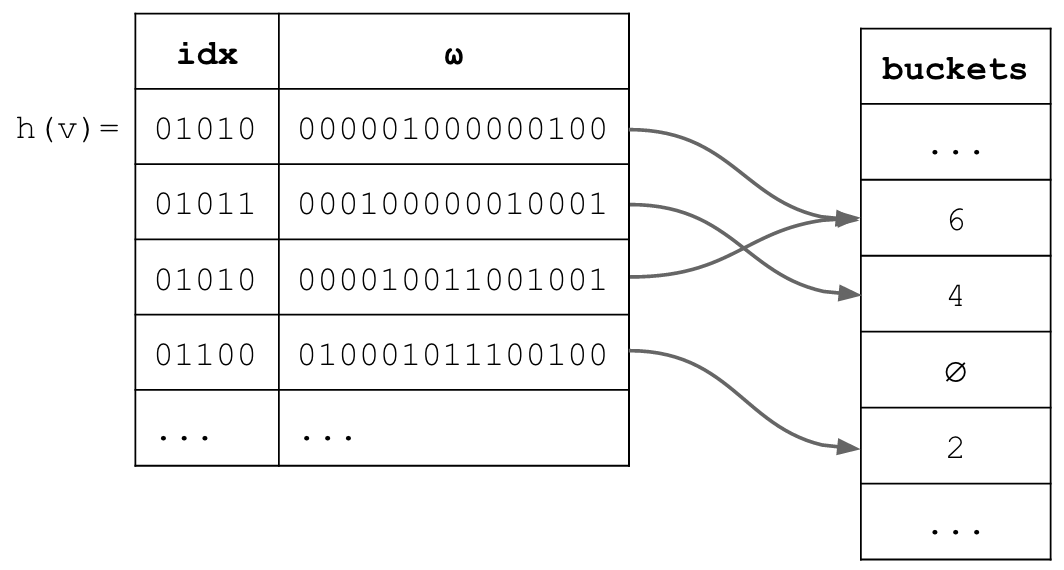
\includegraphics [scale=0.5]  {hyperloglog_buckets.png}
\end{figure}

Memory efficieny : should use less memory for low cardinalities
\begin{itemize}
\item when $n \ll m$, most of registers are never used 
\item => change for a more compact representation
\end{itemize}


\end{frame}

\begin{frame}{What sparse representation}

Key concept : store key/value pairs
\begin{itemize}
\item index as key
\item $\varrho(w)$ as value
\end{itemize}

\begin{figure}[c]
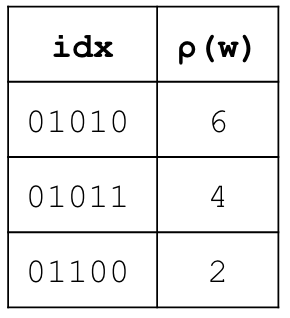
\includegraphics [scale=0.5]  {hyperloglog_list.png}
\end{figure}

Entries can be stored as a single integer (most significant bits for the index, less significant bits for the value)

Sorted list for faster lookups

Convert to the dense representation when the list grows too much : $6\times m < k\times (p + 6)$


\end{frame}


\begin{frame}{Higher precision}

HyperLogLog is less efficient for low cardinalities. 

The sparse representation is used specifically for low cardinalities... why not optimize it ?

=> Why not use a higher precision for this representation ?

=> Using integers, only 6 bits are used for $\varrho(w)$. The other bits can be used for the index. 




$(idx, \varrho(w))$


$6m > k.(p + 6)$

possibilité de switcher
\end{frame}


\begin{frame}{Insertion and merge}
  keeping only the higher value of two pairs with same index, if it's
  not in the list it's 0

  => easier to merge

  maintaining a lsit sorted by indexes
  => and a small buffer(periodically sorted and merged with the list) to make quick insertion

\end{frame}


%% ============================

\begin{frame}{Higher precision}
  
  possibility to increase the precision when only sparse is used =>
  space in registers (biggers indexes)

  use the advantage of the light memory usage
  

\end{frame}

\begin{frame}{Compressed sparsed representation}
\end{frame}


%% ============================

\begin{frame}{Encoding hash values}
\end{frame}

\begin{frame}{Conclusion : Space efficiency}
\end{frame}

\end{document}



(*
% rubber: setlist arguments --shell-escape --enable-write18
Local Variables:
compile-command: "rubber -d slides.tex"
ispell-local-dictionary: "francais"
End:
*)



